% vim:ts=4:sw=4
% Copyright (c) 2014 Casper Ti. Vector
% Public domain.

\chapter{总结}\label{chap:conclusion}
% 中文测试文字。
本章将文中所需要涉及的必要知识进行梳理和阐述,相关概念的定义和简介,不涉及具体证明过程。

\section{PUF工作原理}%
\subsection{工艺涨落}%
芯片制作可分为设计——流片——验证三个大环节,其中设计者输出给流片厂商的是版图信息。版图则对应着制程中每一层掩膜版的图形,具体到晶体管设计上,版图包括了晶体管宽长比,掺杂区域,互联方式等信息,结合工艺常数,决定了晶体管的设计属性。在实际制造中,图形转移过程存在套刻精度、刻蚀精度,以及掺杂过程中的退火控制精度等问题。这些操作在实际中存在不可避免的随机误差和系统误差,而随机误差根本上来源于测量系统的局限性,即永远不可能准确测量原子的位置和速度信息。而误差的累积则造成了工艺涨落,即流片后的晶体管属性与设计属性存在偏差,而其中随机误差的累积则造成设计上属性相同的晶体管在流片后必定存在偏差,也即不匹配,下一节将详细说明如何利用由工艺涨落带来的不匹配。
\subsection{信息转换}
由于无法控制工艺涨落的具体数值,也无法预测涨落的大小,因此``芯片制作''这个物理过程符合PUF所要求的``可测不可知''的物理系统,接下来阐述如何给出工艺涨落的观测点。

\begin{figure}[htb!]
\centering
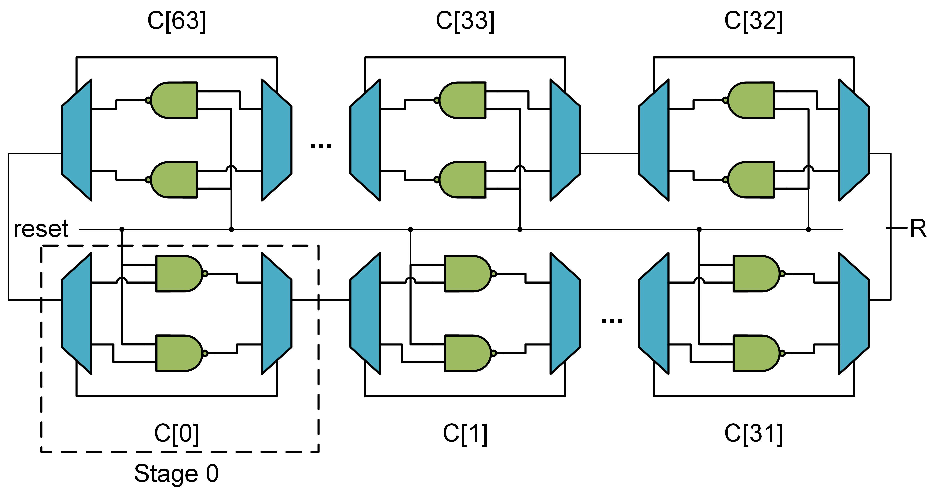
\includegraphics[width=\linewidth]{BRPUF}
\caption{延迟-仲裁型PUF}
\label{fig:arb-puf}
\end{figure}
 
图 2 锁存式PUF

PUF将工艺参数转换为可输出的电压或电流信号。如\ref{fig:arb-puf}所示,其中每个反相器和相邻反相器之间的布线在设计上是全等的,但工艺涨落使得反相器中晶体管导电能力必有差异,那么反相器 $ I_0 $ 的信号延迟 $ \Delta t_0 $ 和 $ I_1 $ 的信号延迟 $ \Delta t_1 $ 定满足关系 $ \Delta t_0-\Delta t_1\neq 0 $ ,当输入一个上升沿信号 $ u(t) $ 后, A-C, A-D 的延迟分别是 $ T_0,T_1 $ ,仲裁器负责判断C节点和D节点信号跳变的先后,一个典型的D触发器即可满足仲裁功能。若C点信号先于D点上跳,则仲裁器输出逻辑``1'',反之则输出逻辑``0''。由于在得到输出之前并不知道每个反相器的实际延迟,所以不能预测仲裁器的输出,而且每一块相同设计芯片之间的输出也因涨落分布的不同而有差异,因此这样的电路逻辑完成了从工艺涨落到电平信号的信息转换。

又如图2所示,两个反相器及布线在设计上是全等的,上电初始电路处于亚稳态,由于实际的反相器存在偏差,导致其中一个节点的充电电流稍大于另一个节点,使得电路大概率由亚稳态向其中一个稳态过度,此大概率得到的稳态也是工艺涨落的体现,这样的电路也完成了从工艺涨落到存储逻辑值的信息转换。值得注意的是,这里使用了``大概率''的说法,是因为在由亚稳态到稳态的弛豫时间中,存在噪声干扰,从而导致电路向工艺无关的方向变化,这是PUF设计中不愿看到的事情。有关PUF稳定性的问题,参见\ref{sec:puf_security}节。
\subsection{Weak PUF和Strong PUF}
类似于\ref{fig:arb-puf}和图 2中的电路,利用物理过程的不可控和不可预测性,表达一位或多位稳定信号的系统被称为物理不可克隆函数(Physically Unclonable Function),其不一定局限于硅基电路,事实上, PUF 概念的首次提出是在光学系统上实现的。

如果将图2中的结构排成阵列,加上行列选择和译码电路,则构成了类似 SRAM 的阵列,通过不同的``地址''信号可以输出不同的单元信息,像这样的``地址信号''在 PUF 中被称为激励(Challenge),输出信号被称为响应(Response)。每一个响应都由一个激励相对应,将它们合称为激励-响应对(C-R Pair, CRP)。

定义:若一个 PUF 的激励响应对很少,则称其为 Weak PUF;反之,激励响应对数量级非常多的则称为 Strong PUF。

Weak PUF 没有对外的 IO 接口,以防被穷举,直接将生成的信号送入后续逻辑;Strong PUF 存在对外的 IO 接口,允许通过输入不同的激励得到一组响应,而 CRP 集合的元素量级决定了不可能穷举完所有的 CRP。

可以看出 Weak PUF 和 Strong PUF 只是人为地划分,没有明确界限,相较而言,目前以 Strong PUF 的研究和应用居多。
\subsection{评价指标}
PUF(这里特指 Strong PUF,后同)可以用以下几个特定指标衡量:
\begin{itemize}
\item 随机性——对任何一个 CRP 集合的子集,响应(简称R,后略)的分布应尽可能满足平均分布;
\item 独特性——对任何一个特定的激励(简称C,后略),一组 PUF 的R的分布应尽可能满足平均分布;
\item 可靠性——对同样的激励在不同环境温度、电源电压下重复操作应给出相同或大概率相同的响应;
\item 安全性——应对各种已知攻击,详见下一节。
\end{itemize}

除此之外,还有电路通用的面积、功耗、速度等指标,但特定指标优先级高于通用指标。

下面给出1-3指标的数学定义:

设C集合$ {c_i} $,R集合$ {r_i} $,$ r_i=f(c_i) $,若$ R={0,1} $,则随机性可以表征为:
\begin{equation}
Rand=\frac{1}{N}\cdot\sum^{N}f(c_i)
\end{equation}
N为 CRP 测试集元素总数,随机性期望值为0.5,表明响应应在随机选取的激励下呈平均分布;

独特性表征为:
\begin{equation}
Uniq=\dfrac{2}{M(M-1)}\sum_{i=1}^{M}\sum_{j=i+1}^{M}\frac{HD(P_i,P_j)}{N}
\end{equation}
\begin{equation}
P_i=<f_i(c_0),f_i(c_1),...,f_i(c_n)>
\end{equation}
其中M为测试PUF设备总数,N为测试激励总数,$ P_i $为第i个设备N个激励响应组成的向量,$ HD(P_i,P_j) $指$ P_i,P_j $之间的汉明距离。
独特性期望值为0.5,表明任意激励的响应在不同设备间应呈平均分布;

可靠性表征为:
\begin{equation}
Reliability=\dfrac{1}{MN}\sum_{j}^{M}\sum_{i}^{N}|f(c')-f^{(j)}(c_i)|
\end{equation}
其中N为测试激励总数,$ M $为测试重复次数,$ c’ $为参考激励,保持不变。可靠性期望值为0。
\section{PUF安全性问题}\label{sec:puf_security}
\subsection{物理模型}
虽然不能精确模拟流片时的掺杂、退火等行为,但是还是可以从宏观上表征一个PUF的行为,成这种方式为建模。通常可以将门级电路的驱动能力、延时等抽象为一个平均值W,将R视为C和W的映射$ R=f(C,W) $。同时,一个好的物理模型有助于快速且准确的仿真验证。
\subsection{参数拟合}
由于 Strong PUF 开放IO端口的特点,若根据攻击者已掌握的一组 CRP 子集,根据建模特点,用机器学习算法拟合出抽象参数$ W $,便可将$ C,W $带入模型中得到 CRP 全集,根据预测率的高低可确定模型建立是否准确抽象了 PUF 的特点。严格来讲,如果一类 PUF 可以被准确抽象出模型,则称该 PUF 是不安全的。但考虑到不是所有模型都能在有限时间内拟合出参数,所以一般认为在特定场合可接受的时间内不能被拟合出参数的 PUF 是安全的。
\section{机器学习算法简介}
\subsection{支持向量机}
支持向量机(Support Vector Machine,SVM),是一种经典的模式识别算法,是 Bell 实验室的 Corinna Cortes 和 Vladimir Vapnik 于1995年首先提出的算法,后经改进,广泛应用于非线性函数拟合,模式识别等机器学习应用中。

SVM 的基本思想是将输入数据映射到一个n维空间中,找到n维空间中的一个超平面能将测试数据集划分开,则该平面将整个空间划分为二,对应着两类不同的数据。

下面我们给出线性SVM的描述。考虑在n维空间中存在m个特征向量$ x_1,x_2,x_3,…,x_m $,每个向量具有一个标签(label)``0''或者``1'',期望找到一个超平面(Hyperplane)
\begin{equation}
g(x)=w'x+b=0
\end{equation}
其中w和b是超平面的系数向量。$ g(x) $可以将特征向量分为两类,使得标签``1''向量都满足$ g(x_i )>0 $,而标签``0''向量都满足$ g(x_i )<0 $。定义
\begin{equation}
\gamma=\frac{g(x)}{||w||}
\end{equation}
为向量x到超平面$ g(x)=0 $的几何距离,其中
$ ||w||=\sqrt{w_1^2+w_2^2+...+w_n^2} $
是系数向量w的范数。
为了增加分类的可信度,我们需要找到一个超平面,使得所有特征向量到该超平面的几何距离最大。

事实上并不是所有的数据都是线性可分的,即不存在一个超平面可以将数据集按标签分开。因此非线性 SVM 的做法通常是:
将数据由n维空间映射到n+k维,使得在n+k为空间中数据线性可分。
\subsection{SVM与PUF}
如果PUF的模型是$ r=f(c)=sgn(\omega'c+b) $的形式,其中r是响应,c是激励,$ \omega $是PUF内在属性,$ sgn() $是一个符号函数。可以看出$ g(c)=\omega'c+b=0 $便类似于SVM中的超平面,在c所在空间中,$ g(c) $将向量c按标签r分为了两类。通过SVM找到使$ \gamma=\frac{g(c)}{||\omega||} $最大的$ \omega $,以使模型达到最大可信度。SVM的求解过程在Matlab中以SMO算法封装实现,而且求解过程并不是本文的关注点,所以不在这里赘述。
\section{相关工作}
\subsection{仲裁型PUF}
图 1展示了一个简单的仲裁型 PUF,图 3是一个完整的仲裁型 PUF。其中激励$ c_i $控制双口交换器使得
\begin{eqnarray}
O_0=c_i?I_1:I_0\\
O_1=c_i?I_0:I_1
\end{eqnarray}
这样不同的激励选定了不同的两条数据通路做延迟对比,使得CRP空间有$ 2^n $个元素。
 
图 3 仲裁型PUF

将每一个交换器抽象为4条通路,设每条通路延迟分别为$ p_i,q_i,r_i,s_i $(如图 4所示),信号到达输入的时间分别为$ t_1(i),t_2(i) $,输出的时间分别为$ t_1(i+1),t_2(i+1) $,则有
\begin{eqnarray}\label{eq:apuf-cell}
t_1(i+1)=c_i?t_2(i)+r_i:t_1(i)+p_i \\
t_2(i+1)=c_i?t_1(i)+q_i:t_2(i)+s_i
\end{eqnarray}

图 4 双口交换器模型

为了方便数学推导,将逻辑``0''记为-1,将逻辑``1''记为+1,则``异或''等价``乘''运算,故\ref{eq:apuf-cell}可化为
\begin{eqnarray}
t_1(i+1)=\frac{1+c_i}{2}(t_2(i)+r_i)+\frac{1-c_i}{2}(t_1(i)+p_i) \\
t_2(i+1)=\frac{1+c_i}{2}(t_1(i)+q_i)+\frac{1-c_i}{2}(t_2(i)+s_i)
\end{eqnarray}
两式做差得:
\begin{equation}
\delta (i+1)=t_1(i+1)-t_2(i+1)=-c_i\delta(i)+\frac{r_i-q_i+p_i-s_i}{2}+\frac{c_1}{2}(r_i-q_i-p_i+s_i)
\end{equation}
求解此递推关系式最终可得:
\begin{equation}
\delta(n)=p'd
\end{equation}
其中向量$ p=<p_0,p_1,…,p_n> $,$ p_i=\Pi_{k=i+1}^{n}c_k $,向量$ d=<\alpha_1,\alpha_2+\beta_1,…,\alpha_n+\beta_(n-1),\beta_n> $,$ \alpha_i=\frac{r_i-q_i-p_i+s_i}{2},\beta_i=\frac{r_i-q_i+p_i-s_i}{2} $,并定义$ p_n $为常数1。由于$ r=f(c)=sgn[\delta(n)] $,所以存在n维空间上的超平面$ p'd=0 $将特征向量p按r标签分开。在这里p是向量c在同维空间中的一个映射,而向量d代表了每个交换器的延迟时间,是PUF的本征属性。

通过一组已知的CRP子集,我们可以确定一组向量d,用SVM算法找到具有最大可信度的d向量,作为延迟时间的估值,这样便推导出了仲裁型PUF的模型,对于未知响应的激励$ c’ $,根据$ sgn(p'd) $可预测其响应。根据文献\supercite{chen2011bistable}的数据,当训练集大小超过2000时,预测准确率在95\%以上。
\subsection{仲裁型PUF的改进}
因为仲裁型PUF的观测点——延迟时间的累加是线性过程,所以容易建立适合SVM算法的模型。在文献【】中作者提出了改进方案——前馈仲裁型PUF(如图 5),用中间值$ sgn[\delta(k)] $作为交换器的控制信号,如果用同样的思路建立模型,那么在模型表达式中存在非线性函数sgn,不能再直接使用SVM算法求解代表延迟的d向量。
 
图 5 前馈仲裁型PUF

\subsection{双稳态环路PUF}
2011年Qingqing Chen等人在会议 Hardware-Oriented Security Transaction 上提出了一种新的PUF,双稳态环路型 PUF(Bistable Ring PUF,如图 6)。 BRPUF采用了偶数级反相器级联构成回路具有双稳态的特性构建PUF的观测点,具有新颖性,并且作者声称其环路具有非线性结构,较传统仲裁型PUF安全性更高。
截止本文撰写时,仅有 Qingqing Chen 本人在文献\supercite{chen2012characterization}中对 BRPUF 做了特性分析; D. Schuster 和 R. Hesselbarth 对 BRPUF 用单层神经网络进行建模。\supercite{test-en}
 
图 6 双稳态环路型PUF

\section{本章小结}
